\clearpage
\section{Oblivious Transfer with Discrete Variables}

\begin{tcolorbox}	
\begin{tabular}{p{2.75cm} p{0.2cm} p{10.5cm}} 	
\textbf{Student Name}  &:& Mariana Ramos\\
\textbf{Starting Date} &:& September 18, 2017\\
\textbf{Goal}          &:& Oblivious transfer implementation with discrete variables.
\end{tabular}
\end{tcolorbox}

Oblivious Transfer (OT) is a fundamental primitive in multi-party computation. The one-out-of-two OT consists in a communication protocol between Alice and Bob. At the beginning of the protocol Alice has two messages $m_1$ and $m_2$ and Bob wants to know one of them, $m_b$, without Alice knowing which one, i.e. without Alice knowing $b$, and Alice wants to keep the other message private, i.e. without Bob knowing $m_{\bar{b}}$. therefore two conditions must be fulfilled:
\begin{enumerate}
	\item{The protocol must be concealing, i.e at the beginning of the protocol Bob does not know nothing about the messages sent by Alice, while at the end of the protocol Bob will learn the message $b$ chose by him.}
	\item{The protocol is oblivious, i.e Alice cannot learn anything about bit $b$ and Bob cannot learning nothing about the other message $m_{\bar{b}}$.}
\end {enumerate}

\subsection{OT Protocol Detailed}


First of all, we have to know if Bob is honest or not. In order to get this information Alice will test Bob's honesty.

Let $+$ the rectilinear basis and $\times$ the diagonal basis, where $+$ matches the bit $0$ and $\times$ matches the bit $1$.
\begin{enumerate}
	\item{Alice picks a random basis $a[i]$ and a random state $g[i]$ for each photon \textit{i}. Then, Alice sends to Bob the photons \textit{i} (where $0\le i \le n$) with polarizations are given by $a[i]$ and $g[i]$.}
	\item{Also Bob randomly chooses the basis $b[i]$ according to which he will make the measurements. Next, he measures the photons \textit{i} through basis $b[i]$ and records the data in an array $h[i]$, where $h[i]$ can take values $0$ or $1$ according to the basis that were chosen. Then he makes a commit of all \textit{n} pairs $(b[i],g[i])$ to Alice.}
	\item{After receive Bob's commitments, Alice randomly chooses some positions of the Key's array and tests the basis committed by Bob. If any \textit{i} values reveal $a[i]=b[i]$ and $g[i] \neq h[i]$, Alice immediately stops the protocol, otherwise she accepts the commitment and the protocol continue.}
\end{enumerate}

At this time, we can assume that Bob is honest.
\begin{enumerate}
	\item{First, Alice sends through a classical channel the basis \textbf{a[i]} to Bob.}
	\item{Bob chooses two subsets $I_{0}$ and $I_{1}$ which represents the set of positions which Bob was wrong, i.e the basis chosen by him is different of the basis chosen by Alice $(a[i]\neq b[i])$,  and the positions he has succeeded, i.e the basis chosen by him is the same of the basis chosen by Alice, respectively. He sends through a classical channel this subsets in a random order, $\{ I_{0},I_{1} \}$ or $\{ I_{1},I_{0} \}$.}
	\item{Alice sends to Bob the two messages encrypted according to the sets sent by Bob in the previous step.}
	\item{Bob receives the two messages, though he only may has learnt one of them.}
\end{enumerate}

\subsection{OT Protocol Example}

Let's look in a more specific example.

Let $m_{1}: [1 1 0]$ and $m_{2}:[0 0 1]$ the two messages sent by Alice.

Alice starts picking random keys and save them in an array $g[i]$. Next, she picks random basis and saved them in an array $a[i]$. At this time, we have two arrays where each position has a key value and a basis value.
At the same time, Bob also picks random basis and saves the values in an array $b[i]$.
When they have made all their choices, Alice sends to Bob her basis $a[i]$ and then Bob will check which basis match with his choices.

\begin{table}[H]
\centering
\begin{tabular}{c|c|c|c|c|c|c|c}
\textbf{\textit{i}}         & 1 & 2 & 3 & 4 & 5 & 6      \\ \hline
\textbf{\textit{Keys, g[i]}}  & 0 & 1 & 0 & 1 & 1 & 1     \\ \hline
\textbf{\textit{Alice's basis, a[i]}} & + & + & $\times$ &+ & $\times$ & $\times$ \\ \hline
\textbf{\textit{Bob's basis, b[i]}} & $\times$ & + & + &+ & $\times$ & + \\ \hline

		 & \underline{0} & 1 & \underline{1} & 1 & 1 & \underline{0} \\ \hline
\end{tabular}
\end{table}

With this result Bob picks two new subsets, $I_{0}$ with the positions $i$ where he was wrong about the basis and $I_{1}$ with the positions $i$ where he has succeeded with his choices.

\begin{center}
$I_{0} = \{ 1,3,6 \}$ - Positions of wrong choices\\
$I_{1} = \{ 2,4,5 \}$ - Positions of right choices
\end{center}

Bob sends to Alice a new set $ \{ I_{0},I_{1} \}$ or $\{ I_{1}, I_{0}\}$ randomly ordered. Alice receives $\{ I_{i}, I_{\bar{i}}\}$ and sends to Bob $\{ m_{1}, m_{2}\}$ encrypted with the basis values which match with the positions $i$ sent by Bob:

$$m_{1} \oplus{} \{ 1 1 1 \} = \{ 0 0 1\}$$
$$m_{2} \oplus{} \{ 0 0 1 \} = \{ 0 0 0\}$$

After Bob receives the encrypted messages from Alice, he only is able to decrypted the message he wants, in this case message 1, as we may see bellow:
\begin{center}
$\{ 0 0 1\} \oplus{} \{ 1 1 1\} = \{ 1 1 0\} $: Message 1 $\surd$ \\
$\{ 0 0 0\} \oplus{} \{ 0 1 0\} = \{ 0 1 0\} $: Message 2 $\times$ \\
\end{center}

At the end, Bob was only able to learn one of the messages and Alice still does not know which message Bob has learnt.

\subsection{Simulation}

First of all, the protocol will be simulated and then a experimental setup will be built in the laboratory.

\begin{figure}[H]
	\centering
	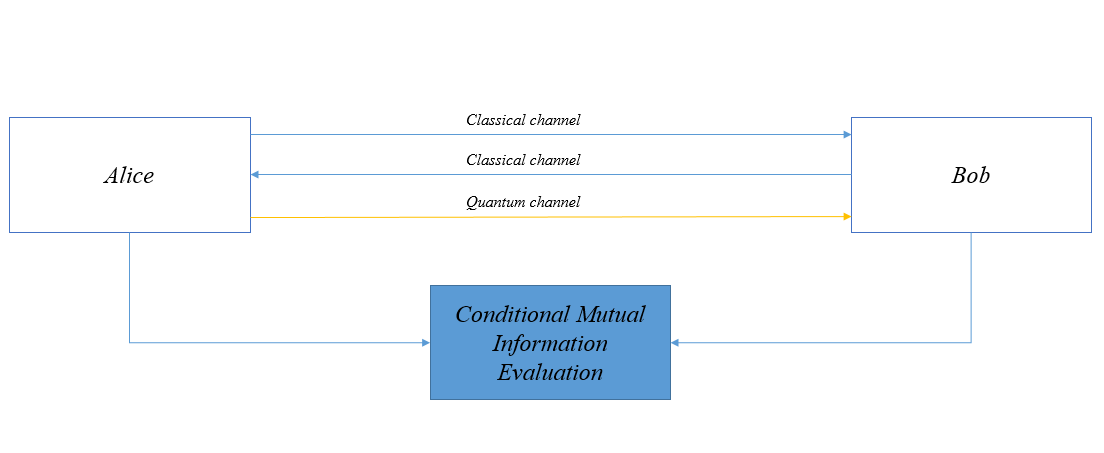
\includegraphics[width=1.0\textwidth, height=11cm]{./sdf/ot_with_discrete_variables/figures/SetupOt.png}
	\caption{Experimental Setup}\label{experimentalsetup}
\end{figure}

As one may see in figure \ref{experimentalsetup} this simulation will have three block. Two of them are Alice and Bob and they are connected through two classical channels and one quantum channel. In addition, a third block will be performed for the calculation of \textit{Mutual Information}. The mutual information (MI) between Alice and Bob is defined in terms of their join distribution.

\begin{figure}[h]
	\centering 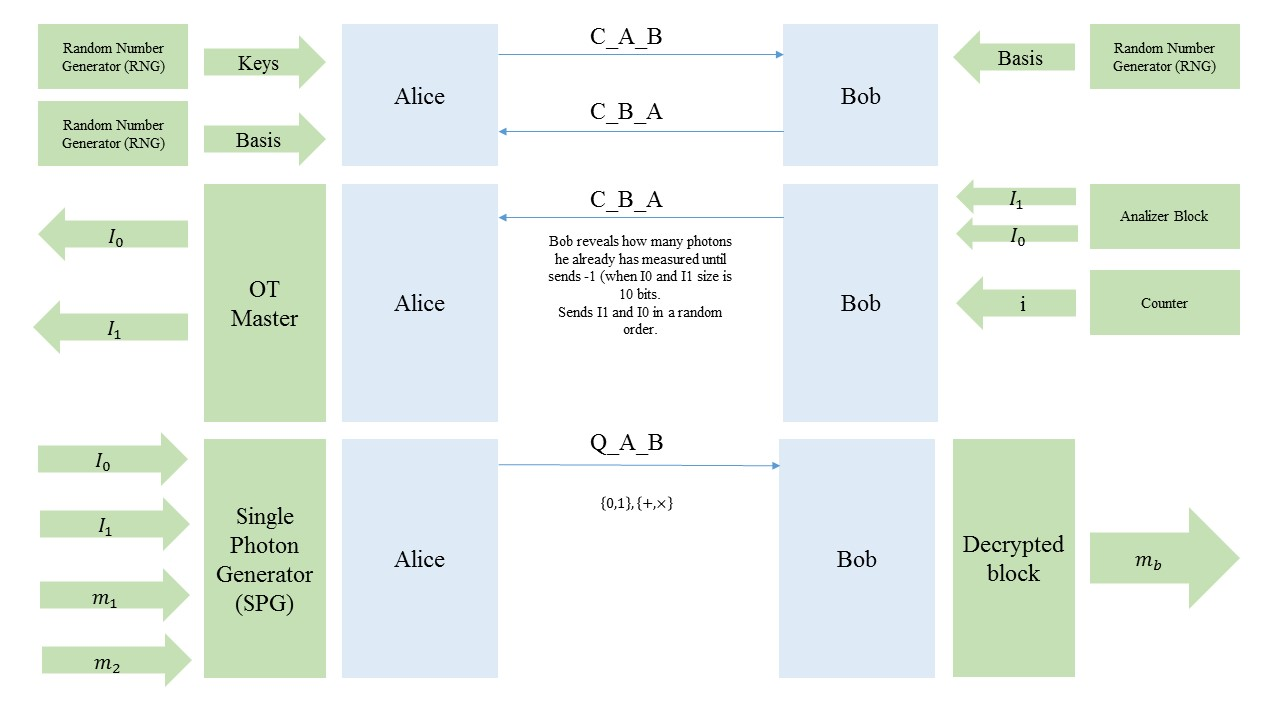
\includegraphics[width=1.1\textwidth,height=9cm]{./sdf/ot_with_discrete_variables/figures/DiagramBlock_Simulation.jpg}
	\caption{Functional Block Diagram}\label{functionalblockdiagram}
\end{figure}

In figure \ref{functionalblockdiagram} is presented the block diagram of the simulation that will be performed. There are two sides (Alice and Bob) and three channels throughout which they will communicate. For classical tasks Alice must have two \textit{Random Number Generators} in order to generate random keys and basis. Likewise, Bob also need to generate the basis through which he will measure the received photons. Next, Bob must have two more blocks, one to analyze and process whether the basis information received by Alice match with his basis information, and another block for photons count. Furthermore, Alice must have a block for \textit{Single Photon Generator} which receives four inputs to encrypt the photons to be sent. Finally, Bob has a block to decrypt messages received by Alice.

\subsection{Experimental}
In figure \ref{quantumchannelcommunication} is presented the experimental setup to be performed in the lab.

\begin{figure}[H]
	\centering 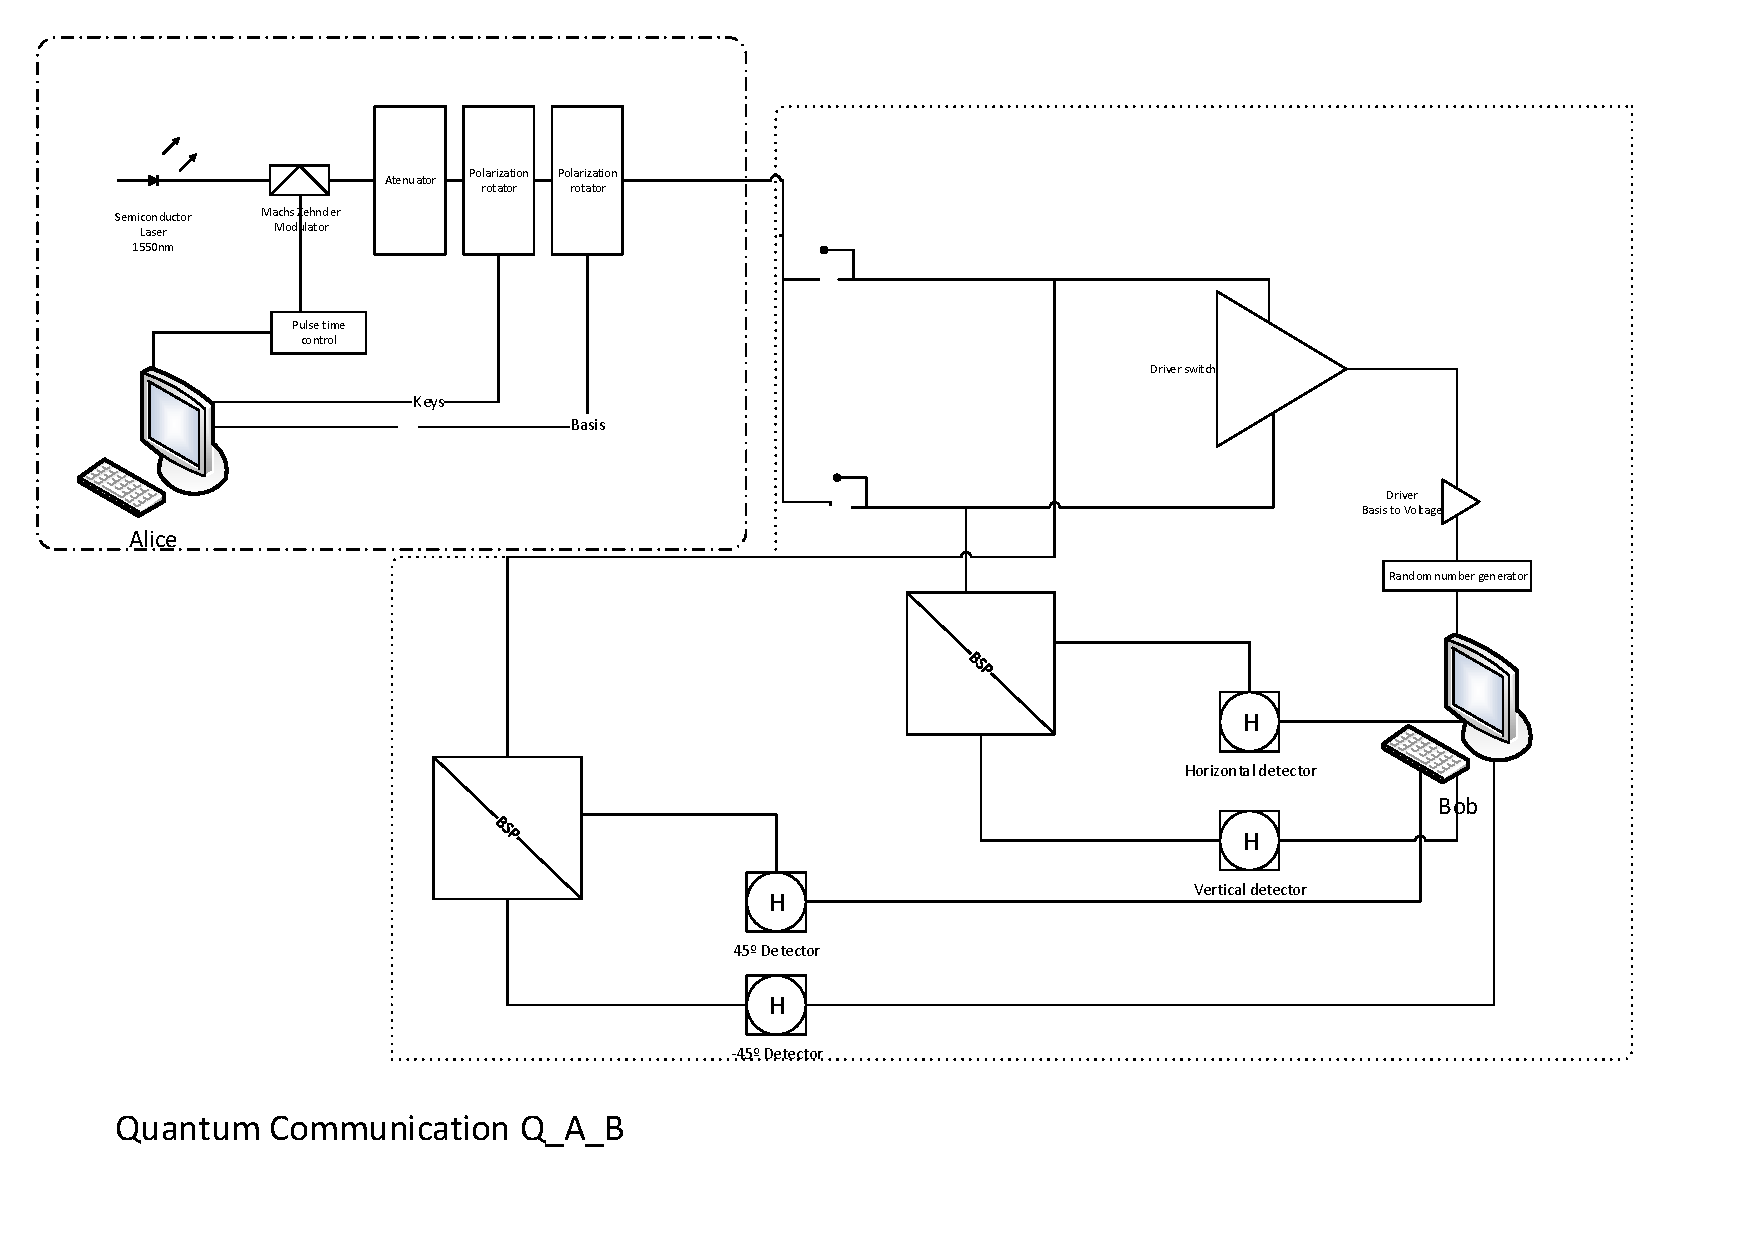
\includegraphics[width=1.2\textwidth,height=12cm]{./sdf/ot_with_discrete_variables/figures/OT_experimental_setup.pdf}
	\caption{Quantum communication diagram}\label{quantumchannelcommunication}
\end{figure}